\rchapter{Parallel Setup}

\section{Introduction}

Gyrokinetic equations are defined in at least four dimensions. This means that even if a small number of points is used in each dimension, the resulting grid will have a very large number of points. In addition the non-linear nature of the equation means that for most dimensions, an accurate solution cannot be obtained from a very small number of points. Operations on such a high volume of data can be very time consuming. It is therefore important to ensure that parallelisation is used wherever possible.

Parallelisation allows independent calculations to be carried out simultaneously. This decreases the time required to calculate the final solution as the solution at multiple points in the data can be calculated simultaneously. For this method to be effective, it is important that as much of the calculation as possible can be carried out independently. If data stored on a different process is required to complete the calculation then the exchange of data will dramatically increase the overhead, slowing down the calculation time. This can negate the improvement achieved by parallelisation and should therefore be avoided wherever possible. This means that if a calculation requires values from multiple points along one dimension, then ideally that dimension should not be distributed.

This highlights a second consideration: the organisation of the data in memory. Different configurations of the data can lead to different memory latency. If data is accessed contiguously then the loading of cache lines and prefetching (which can be carried out easily by the system as the access pattern is easily recognisable) will ensure that the subsequently required data is already found on a cache. This is important as cache misses can be very costly. The further the data must travel before it can be used, the greater the latency. Optimal memory access is especially important as calculations are often memory-bound rather than compute-bound due to the increase in CPU power following Moore's law and the lack of improvement in memory latency.

It is therefore important to manage access to data structures in an efficient way to ensure that calculations can be carried out as quickly and easily as possible. This should be carried out using parallelisation as well as an optimal arrangement of the data in memory.

In this chapter effective ways of managing the data to fulfil these criteria will be examined.

\section{Choosing layouts}

The arrangement of the data in memory depends on the requirements of the calculations. The screw-pinch model with cylindrical geometry is characterised by 3 operators which arise from the following three advection equations:

\begin{align}
 \partial_t f + v_\parallel \nabla_\parallel f &= 0 \label{eq::Advection1}\\
 \partial_t f + \nabla_\parallel \tilde{\phi} \partial_{v_{\parallel}} f &= 0 \label{eq::Advection2}\\
 \partial_t f + \{\tilde{\phi}, f\} &= 0 \label{eq::Advection3}
\end{align}

Equation \ref{eq::Advection1} leads to an operator which acts on the particle distribution function f, along the flux surface. This surface is defined on $\eta_2$ and $\eta_3$ so the memory access for these variables ought to be contiguous for this operator. Equation \ref{eq::Advection2} leads to an operator which acts on the distribution function along the velocity or $\eta_4$. Therefore  the memory access for $\eta_4$ ought to be contiguous for this operator. Equation \ref{eq::Advection3} leads to an operator which acts on the distribution function along the poloidal surface. This surface is defined on $\eta_1$ and $\eta_2$ so the memory access for these variables ought to be contiguous for this operator.

Evidently it is not possible to find a structure which is optimal for all three of these operators, however given the amount of calculation involved with each step it is reasonable to change layout between each operator. This has been done previously by Latu et al, 2007 \cite{Gysela5D}. A setup must therefore be found such that the following requirements are met:

\begin{tcolorbox} [enhanced,title=Requirements,attach boxed title to top left={xshift=10pt,yshift=-\tcboxedtitleheight/2},boxed title style={size=small}]

\begin{enumerate}
 \item The number of processes that can be used is maximised \label{Condition Max nprocs}
 \item The dimensions used by the operator are not distributed  \label{Condition distribution}
 \item The dimensions used by the operator are contiguous \label{Condition contiguous}
 \item The number of MPI messages sent and received is minimised \label{Condition MPI overhead}
 \item The memory required is minimised \label{Condition memory}
 \item After setup no memory is allocated \label{Condition allocation}
 \item As little copying of data as possible is used \label{Condition copying}
\end{enumerate}

\end{tcolorbox}

With no other requirements, the maximum number of processes possible is equal to the number of grid points. However requirement \ref{Condition distribution} inhibits requirement \ref{Condition Max nprocs}. Thus the maximum number of processes possible for a given layout is the product of the number of points in each dimension not being used by the operator. In order to achieve a good load balance, the number of processes used in each operation should be the same. Thus the maximum number of processes that can be used at any one time is:

$$max\_procs = \min\{n_{\eta_1}\!\!\cdot n_{\eta_4},\, \, \, n_{\eta_1}\!\!\cdot n_{\eta_2}\!\! \cdot n_{\eta_3},\, \, \, n_{\eta_3}\!\!\cdot n_{\eta_4}\}$$

\begin{table}
\centering
 \begin{tabular}{|c|c|}
  \hline
  Dimension & Number of points\\
  \hline
  $\eta_1$ & 256\\
  \hline
  $\eta_2$ & 512\\
  \hline
  $\eta_3$ & 32\\
  \hline
  $\eta_4$ & 128\\
  \hline
 \end{tabular}
 \caption{\label{tab::Grid example} Example configuration of data points}
\end{table}

Using the example setup in table \ref{tab::Grid example}, it can be seen that in this situation the maximum number of processes would be $n_{\eta_3}\!\!\cdot n_{\eta_4} = 4096$. This shows that it does not make sense to distribute this example in more than two dimensions. Even if we tried to take advantage of being able to distribute in three dimensions for equation \ref{eq::Advection2}, it would be unlikely that this would significantly increase the total number of processes that could be used, as in general $n_{\eta_4}\ll n_{\eta_1}\cdot n_{\eta_2}$. In addition it is often the case that $n_{\eta_4}< n_{\eta_1}$ and $n_{\eta_4}<\cdot n_{\eta_2}$ which would mean that no gains in the total number of processes would be made. Thus the increase in complexity does not justify the possible gains. 

The example setup in table \ref{tab::Grid example} also shows that it makes sense to aim for a distribution in two dimensions. The maximum number of processes that can be used in this case ($n_{\eta_3}\!\!\cdot n_{\eta_4} = 4096$) is significantly larger than the maximum number of processes that could be used if the data was only distributed in one dimension ($\eta_4=128$). Therefore the two dimensional distribution is optimal, unless it causes very large overhead thus violating requirement \ref{Condition MPI overhead}.

This therefore leaves us with the possible configurations shown in table \ref{tab::Possible Ordering}. This ordering is such that non-distributed dimensions are always in the final indices, thus satisfying requirement \ref{Condition contiguous}.

\begin{table}[ht]
\centering
 \begin{tabular}{|c|c|}
  \hline
  Accessing scheme & Possible Ordering\\
  \hline
  Flux surface & $(\eta_1,\eta_4,\eta_2,\eta_3)$\\
               & $(\eta_4,\eta_1,\eta_2,\eta_3)$\\
               & $(\eta_1,\eta_4,\eta_3,\eta_2)$\\
               & $(\eta_4,\eta_1,\eta_3,\eta_2)$\\
  \hline
  V-parallel surface & $(\eta_1,\eta_2,\eta_3,\eta_4)$\\
                     & $(\eta_1,\eta_3,\eta_2,\eta_4)$\\
                     & $(\eta_2,\eta_1,\eta_3,\eta_4)$\\
                     & $(\eta_2,\eta_3,\eta_1,\eta_4)$\\
                     & $(\eta_3,\eta_1,\eta_2,\eta_4)$\\
                     & $(\eta_3,\eta_2,\eta_1,\eta_4)$\\
  \hline
  Poloidal surface & $(\eta_3,\eta_4,\eta_1,\eta_2)$\\
                   & $(\eta_4,\eta_3,\eta_1,\eta_2)$\\
                   & $(\eta_3,\eta_4,\eta_2,\eta_1)$\\
                   & $(\eta_4,\eta_3,\eta_2,\eta_1)$\\
  \hline
 \end{tabular}
 \caption{\label{tab::Possible Ordering} Plausible orderings of dimensions in the three different layouts}
\end{table}

In order to simplify the problem, additional restrictions are placed on the setup. Firstly it is assumed that $\eta_2$ is never distributed, as in any case there is only one setup in which it could be distributed. This has no effect on the preceding discussion. In addition it is assumed that $\eta_2$ will always be in the same position in the ordering. As $\eta_4$ must be contiguous for the operator associated with equation \ref{eq::Advection2}, $\eta_2$ must therefore always be in the third position. This leaves two possible orderings. The choice between the two is arbitrary (the only difference is that the ordering in the first and second positions are exchanged). The choice made here can be seen in table \ref{tab::Ordering}.

\begin{table}[ht]
\centering
 \begin{tabular}{|c|c|}
  \hline
  Accessing scheme & Ordering\\
  \hline
  Flux surface & $(\eta_1,\eta_4,\eta_2,\eta_3)$\\
  \hline
  V-parallel surface & $(\eta_1,\eta_3,\eta_2,\eta_4)$\\
  \hline
  Poloidal surface & $(\eta_4,\eta_3,\eta_2,\eta_1)$\\
  \hline
 \end{tabular}
 \caption{\label{tab::Ordering} The chosen ordering for the three different layouts}
\end{table}

Using this ordering, it is important to find a method for changing layouts which respects requirements \ref{Condition memory}, \ref{Condition allocation}, \ref{Condition copying}, and especially \ref{Condition MPI overhead}.

\section{Moving between layouts}

It is clear from the ordering in table \ref{tab::Ordering} that at each change of layout: $\eta_2$ is untouched, one dimension must become distributed, one dimension must become contiguous and one dimension must not be touched unless the number of processes along that axis changes. The problem can therefore be simplified further by assuming that this will not happen. In other words, in a given distribution direction, at any given moment, the data will be distributed over the same number of processes in that direction. The only difference will be which dimension is stored along that axis in memory (ie. for the ordering in table \ref{tab::Ordering}, $\eta_1$ or $\eta_4$ on the first storage axis will each be distributed over the same number of processes).
%In other words, the number of processes available along each axis will remain constant throughout the simulation, and only which variable is represented by that axis will vary.
As $\eta_2$ does not vary the problem can therefore be visualised in three dimensions as shown in figure \ref{fig::Cartesian}. It should be noted that these decisions have removed some flexibility from our system. In particular, it should be noted that it is impossible to move from a poloidal surface to a flux surface without either first changing to a $v_\parallel$ surface or changing the ordering of the variables in the flux surface.


\begin{figure}[ht]
 \begin{center}
 \begin{subfigure}[t]{.45\textwidth}
  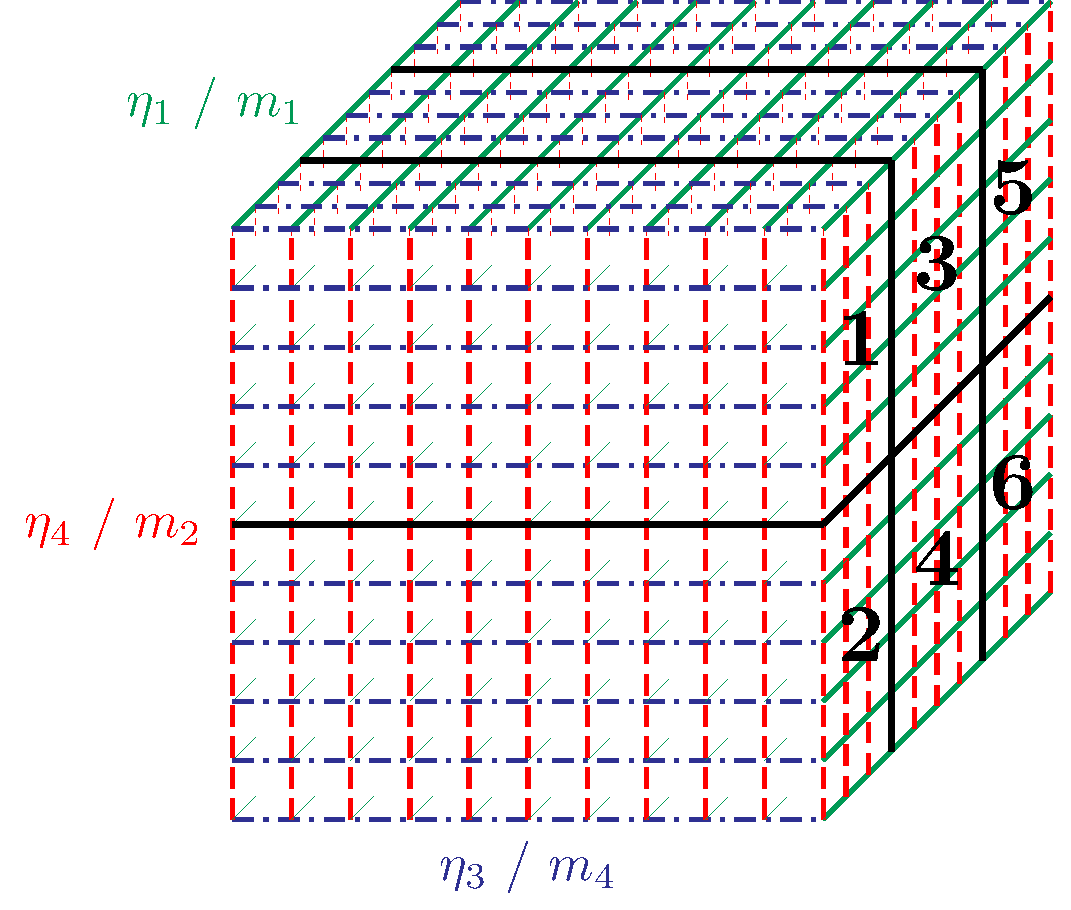
\includegraphics[width=\textwidth]{Figs/ParallelDivision/FluxSurface}
  \caption{\label{fig::FluxSurface}Flux surface - contiguous in z}
 \end{subfigure}
 \hspace{.05\textwidth}
 \begin{subfigure}[t]{.45\textwidth}
  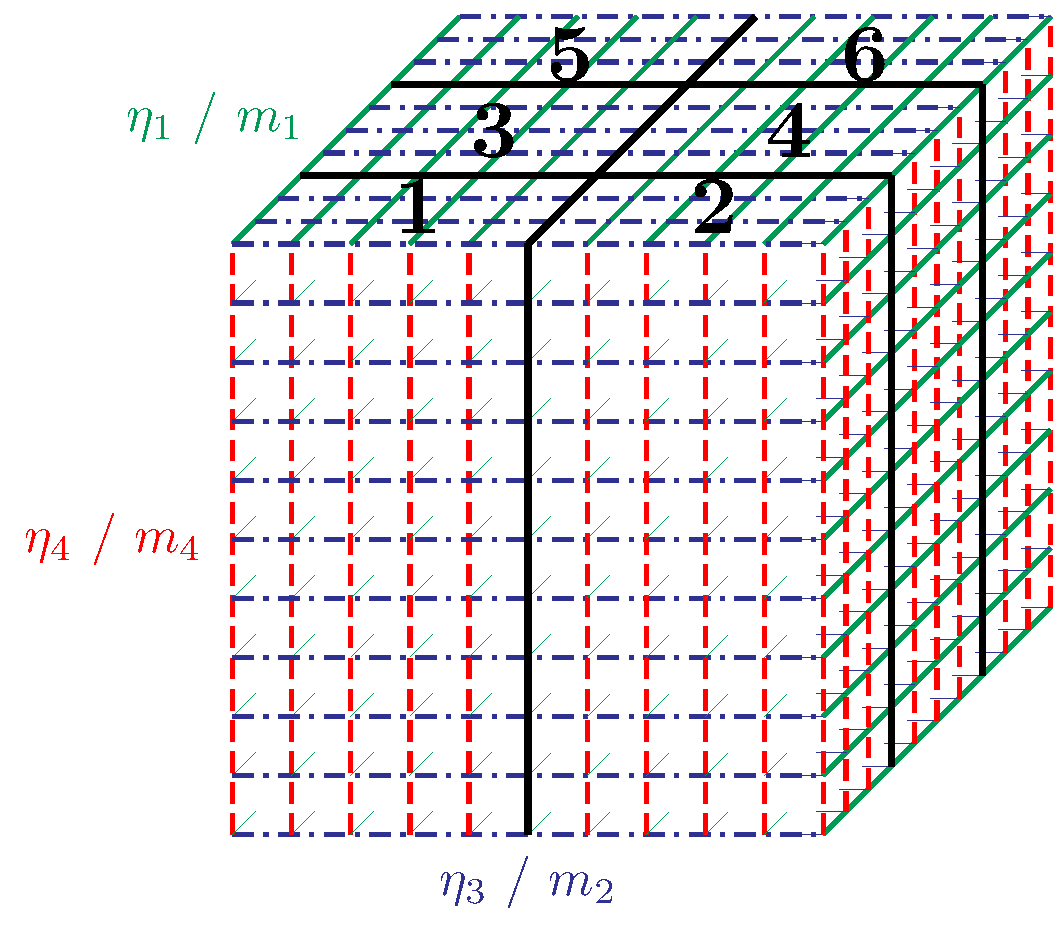
\includegraphics[width=\textwidth]{Figs/ParallelDivision/VParSurface}
  \caption{\label{fig::VPar}$v_\parallel$ surface - contiguous in $v_\parallel$}
 \end{subfigure}
 \begin{subfigure}[t]{.45\textwidth}
  \vspace{1em}
  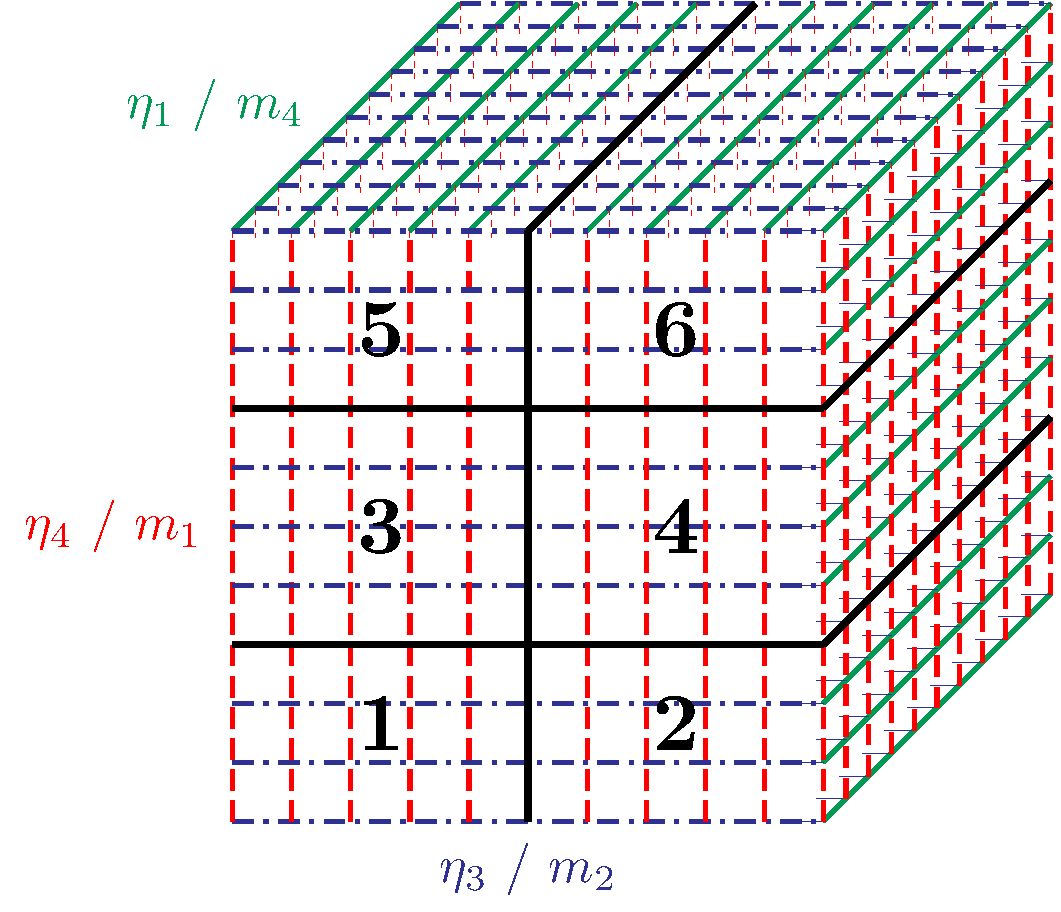
\includegraphics[width=\textwidth]{Figs/ParallelDivision/PoloidalSurface}
  \caption{\label{fig::Poloidal}Poloidal surface - contiguous in r}
 \end{subfigure}
  \caption{\label{fig::Cartesian} 3-D visualisation of the layout change problem. The axis along which the data is stored in memory is indicated by $m_1,m_2,m_4$ ($m_3$ is not represented as it always contains all values of $\eta_2$). Note that the storage axis only changes when the distribution pattern along that axis changes.}
 \end{center}
\end{figure}

Figure \ref{fig::Cartesian} shows three different layouts and allows the viewer to visualise the movement of data between processes during a layout change. Consider the change from the flux-surface layout (figure \ref{fig::FluxSurface}) to the $v_\parallel$ surface layout (figure \ref{fig::VPar}). Process 1 and process 2 must exchange data with one another, however no data is required from any of the other processes. This is also the case for processes 3 and 4, and processes 5 and 6. Similarly when changing from the $v_\parallel$ surface layout to the poloidal surface layout (\ref{fig::Poloidal}) processes 1, 3, and 5 must exchange data only with one another. Indeed, with the conditions imposed each three dimensional layout change is equivalent to multiple independent two dimensional layout changes.

This property can be exploited using an MPI Cartesian grid. This allows the number of messages sent to be greatly reduced thus fulfilling requirement \ref{Condition MPI overhead}. If all processes exchange data amongst themselves, then $p^2$ messages are exchanged,  where $p$ is the total number of processes. In the setup described here, for a grid distributed along a $n \times m$ grid of processes ($nm=p$), changing the variable represented by the first storage axis requires $m n^2$ messages, and changing the variable represented by the second storage axis requires $n m^2$ messages.

In addition the reduced problem can be expressed in one MPI collective command on a sub-communicator: Alltoall. This allows us to use the algorithms provided by MPI rather than relying on multiple point to point messages. This will almost always result in a better optimisation of the code as the MPI implementation can be optimised for hardware.

\subsection{Practical Implementation}

The different layouts each have different memory requirements. This would appear to mean that in order to fulfil requirement \ref{Condition allocation} (after setup no memory is allocated), one array must be allocated for each layout. However this is not ideal as indicated by requirement \ref{Condition memory}. In order to improve this situation, views on numpy arrays are used to access the data. Numpy arrays consists of a 1D array storage and a set of values representing the step-size between consecutive elements in the same dimension. A numpy view is a numpy array where the data has been stored by a different array. Using views therefore allows the allocation of a single one-dimensional array containing the maximum amount of memory required by any given layout. The view then points to a subset of this memory and allows it to be accessed as a multi-dimensional array.

\begin{figure}[ht]
 \begin{center}
 \begin{subfigure}[t]{0.4\textwidth}
  \centering
  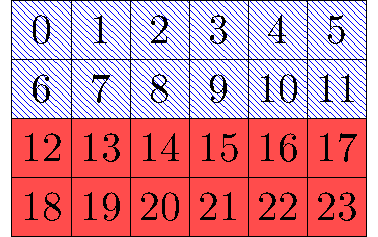
\includegraphics[width=\textwidth]{Figs/SplitConcat2D/Layout1}
  \caption{\label{fig::SplitConcat layout1}Layout 1}
 \end{subfigure}
 \hspace{0.05\textwidth}
 \begin{subfigure}[t]{0.5\textwidth}
  \centering
  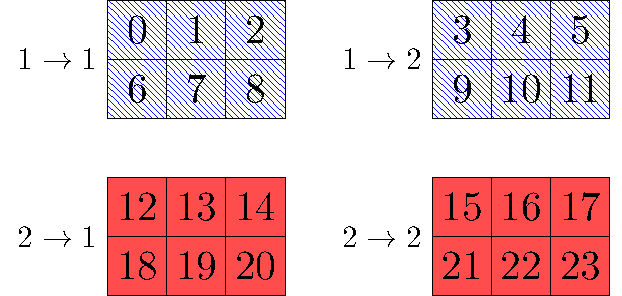
\includegraphics[width=\textwidth]{Figs/SplitConcat2D/SendBlocks}
  \caption{\label{fig::SplitConcat send blocks}Blocks to be sent. These must be copied to a buffer in order to be contiguous by block in memory}
 \end{subfigure}
 \begin{subfigure}[t]{0.5\textwidth}
  \centering
  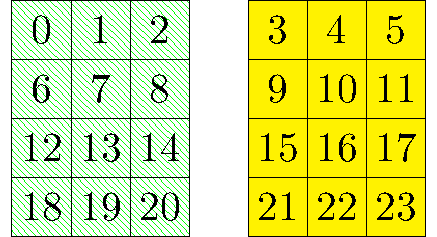
\includegraphics[width=\textwidth]{Figs/SplitConcat2D/RecvLayout}
  \caption{\label{fig::SplitConcat recv blocks}Blocks that are received. These are contiguous but the dimensions are not correctly ordered}
 \end{subfigure}
 \hspace{0.05\textwidth}
 \begin{subfigure}[t]{0.4\textwidth}
  \centering
  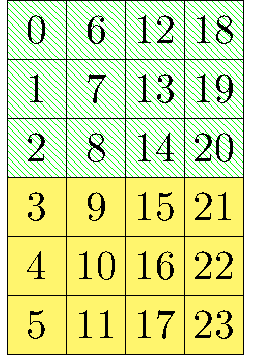
\includegraphics[width=.5\textwidth]{Figs/SplitConcat2D/Layout2}
  \caption{\label{fig::SplitConcat layout2} Layout 2}
 \end{subfigure}
 \begin{subfigure}[t]{\textwidth}
  \centering
  \vspace{1em}
  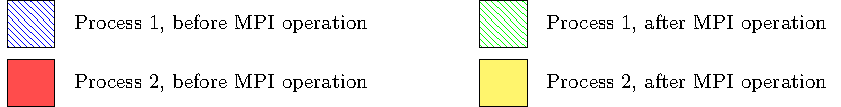
\includegraphics[width=.9\textwidth]{Figs/SplitConcat2D/Legend}
 \end{subfigure}
  \caption{\label{fig::SplitConcat} 2-D visualisation of the layout change algorithm.}
 \end{center}
\end{figure}

When the layout is changed a second array is required for the data to be received. With careful management no additional memory should be required, thus fulfilling requirement \ref{Condition memory}.

Note that the numpy views used for each layout will be different as the dimensions represented by each storage axis change. This can be seen in figure \ref{fig::Cartesian}, but is shown more clearly in figure \ref{fig::Division in memory}.

\begin{figure}[ht]
 \centering
 \begin{subfigure}[t]{0.45\textwidth}
  \centering
  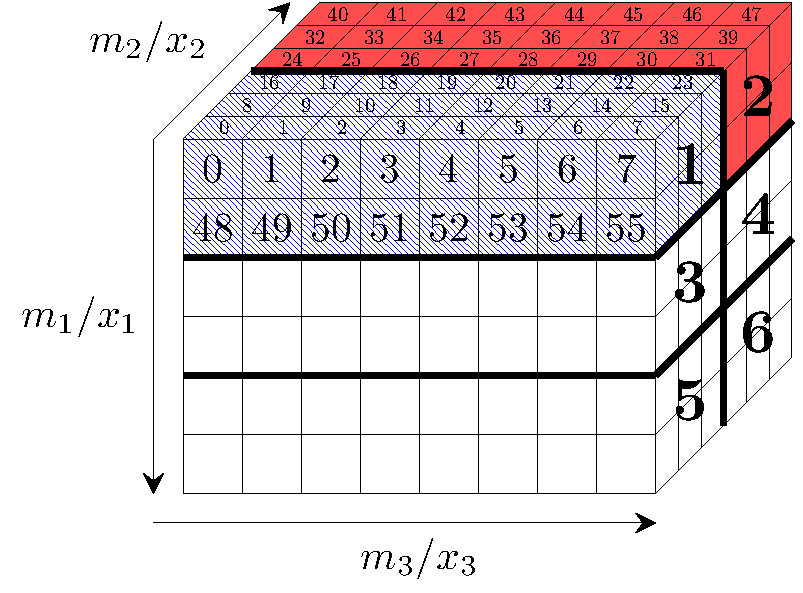
\includegraphics[width=\textwidth]{Figs/DivisionInMemory/FluxSurface}
  \caption{\label{fig::Division in memory Flux} Layout 1}
 \end{subfigure}
 \hspace{0.05\textwidth}
 \begin{subfigure}[t]{0.4\textwidth}
  \centering
  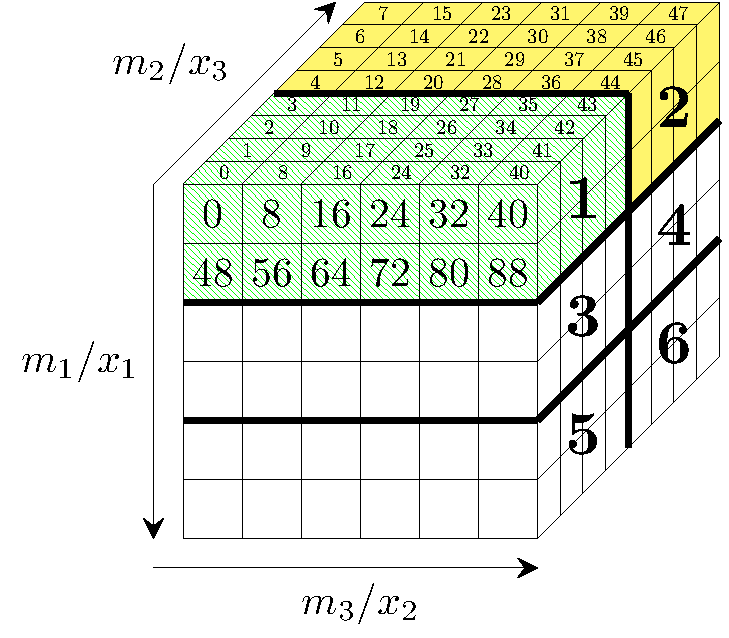
\includegraphics[width=\textwidth]{Figs/DivisionInMemory/VPar}
  \caption{\label{fig::Division in memory VPar} Layout 2}
 \end{subfigure}
 \caption{\label{fig::Division in memory}Different layout arrangements in memory. Note that when the layout changes the shape of the data in memory changes (Colouring is relevant for figure \ref{fig::3D layout change})}
\end{figure}

\begin{figure}[p]
 \begin{center}
 \begin{subfigure}[t]{0.45\textwidth}
  \centering
  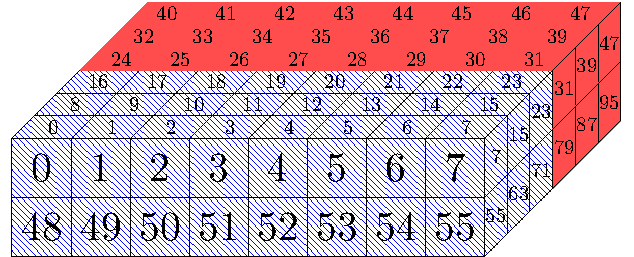
\includegraphics[width=\textwidth]{Figs/SplitConcat3D/Layout1}
  \caption{Layout 1}
 \end{subfigure}
 \hspace{0.05\textwidth}
 \begin{subfigure}[t]{0.45\textwidth}
  \centering
  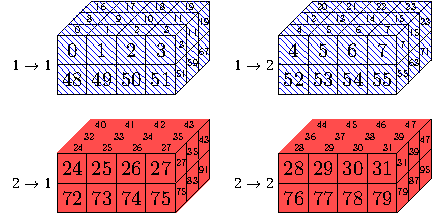
\includegraphics[width=\textwidth]{Figs/SplitConcat3D/SendBlocks}
  \caption{\label{fig::3DSplitConcat send blocks} Blocks to be sent. These must be copied to a buffer in order to be contiguous by block in memory}
 \end{subfigure}
 
 \begin{subfigure}[t]{0.45\textwidth}
  \centering
  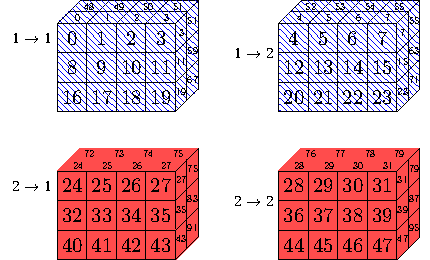
\includegraphics[width=\textwidth]{Figs/SplitConcat3D/TransposedSendBlocks}
  \caption{\label{fig::3DSplitConcat send blocks T}Before sending, the blocks are rearranged so that the axis which was previously distributed becomes the axis with the largest step size (the first axis)}
 \end{subfigure}
 \hspace{0.05\textwidth}
 \begin{subfigure}[t]{0.45\textwidth}
  \centering
  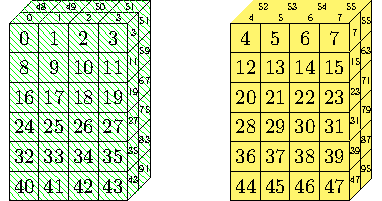
\includegraphics[width=\textwidth]{Figs/SplitConcat3D/RecvLayout}
  \caption{\label{fig::3DSplitConcat recv blocks}Blocks that are received. These are contiguous but the dimensions are not correctly ordered}
 \end{subfigure}
 
 \begin{subfigure}[t]{0.45\textwidth}
  \centering
  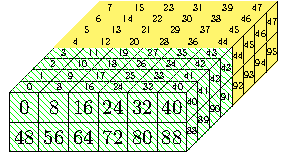
\includegraphics[width=\textwidth]{Figs/SplitConcat3D/Layout2}
  \caption{\label{fig::3DSplitConcat layout2} Layout 2}
 \end{subfigure}
 \hspace{0.05\textwidth}
 \begin{subfigure}[t]{0.45\textwidth}
  \centering
  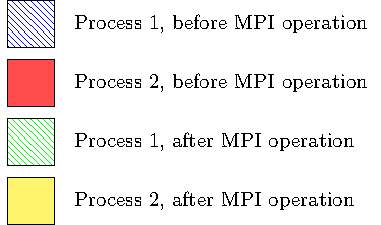
\includegraphics[width=.9\textwidth]{Figs/SplitConcat3D/Legend}
 \end{subfigure}
  \caption{\label{fig::3D layout change} 3-D visualisation of the layout change algorithm. The figure shows the steps for moving the data on processes 1 and 2 from the layout described in figure \ref{fig::Division in memory Flux} to the layout described in figure \ref{fig::Division in memory VPar}}
 \end{center}
\end{figure}

The remaining requirement is requirement \ref{Condition copying} regarding the copying of data. In an ideal implementation the data involved would only be copied once, when it is sent. However unfortunately this is not possible with the layouts described above. The reason for this is illustrated in figure \ref{fig::SplitConcat}. The data is stored in such a way that it is contiguous in memory (figure \ref{fig::SplitConcat layout1}). However this means that the data which will be moved to a different process is not contiguous (figure \ref{fig::SplitConcat send blocks}). As a result a first copy is required before the data can be transmitted. In addition on arrival the data is not ordered correctly (figure \ref{fig::SplitConcat recv blocks}). In two dimensions, this simply means that a transpose is required (figure \ref{fig::SplitConcat layout2}), however in more dimensions the situation is more complicated. The data must be concatenated along the correct storage axis as well as being transposed to the correct shape. The concatenation step is however not required if the dimension to be concatenated is stored along the first storage axis. This is due to the way in which the data is stored in memory.

\begin{algorithm}[p]
 \hspace*{\algorithmicindent} \textbf{Input \, :}
 \begin{minipage}[t]{.8\textwidth}
  A start layout {\em startLayout} and an end layout {\em endLayout} \\
  A memory block {\em Arr} containing the distribution function evaluated in the start layout \\
  An additional memory block {\em Buf} \\
 \end{minipage}
 
 \hspace*{\algorithmicindent} \textbf{Output :}
 \begin{minipage}[t]{.8\textwidth}
  A memory block {\em Buf} containing the distribution function evaluated in the end layout \\
 \end{minipage}

 \begin{algorithmic}[1]
  \STATE Find the axes ({\em ax\textsubscript{concat}},{\em ax\textsubscript{distrib}}) in {\em startLayout} which are exchanged\\ in {\em endLayout}
  
  \STATE Define {\em ax\textsubscript{1}}, the first axis in the {\em startLayout}
  
  \STATE Store views on slices of {\em Arr}, obtained by splitting along {\em ax\textsubscript{distrib}}
  
  \STATE
  
  \FOR{ each (non-contiguous) view }
      \STATE Permute the axes of the view using the permutation: ({\em ax\textsubscript{1}}, {\em ax\textsubscript{concat}})
      %\STATE Transpose the view such that {\em ax1} is the first dimension
      %\STATE Write the (contiguous) transposition into {\em Buf}
      \STATE Write the result (contiguously) into {\em Buf}
  \ENDFOR
  
  \STATE
  
  \STATE {\bf Send} the data from {\em Buf} using Alltoall
  
  \STATE {\bf Receive} the data into {\em Arr}
  
  %\STATE Transpose the dimensions to the order in {\em endLayout}
  
  \STATE Permute the axes of a view on the data, using the permutation:\\ ({\em ax\textsubscript{1}},{\em ax\textsubscript{distrib}},{\em ax\textsubscript{concat}})
  
  \STATE Write the transposition into {\em Buf}
  
 \end{algorithmic}
 \caption{\label{algo::layout change} Algorithm describing the change of layout}
\end{algorithm}

The final algorithm utilises this fact. The data is split along the final storage axis and reordered such that the dimension to be concatenated is first. Thus after the MPI operation the only step required is the reordering of the dimensions.

If the dimension to be concatenated is already stored on the first axis then only the first and last storage axes play a role. As a result the algorithm can be visualised in two dimensions as in figure \ref{fig::SplitConcat}. The reader can convince themselves of this fact by imagining a third axis on figure \ref{fig::SplitConcat} which does not play a role. This shows that the 2-D case can be extended to 3-D if the second dimension plays no role. The N-D case can be summarised to the 3-D case by representing the (N-2) central dimensions by one variable.

If the dimension to be concatenated is not stored on the first axis then the algorithm must be visualised in three dimensions as in figure \ref{fig::3D layout change}. As previously the data which will be moved to a different process is not contiguous (figure \ref{fig::3DSplitConcat send blocks}). During the first copy, which ensures contiguity for sending, the dimensions are also reordered to position the dimension to be concatenated on the first storage axis (figure \ref{fig::3DSplitConcat send blocks T}). The data can then be sent in the same manner as described in the 2-D case. In both cases, the data is not ordered correctly on arrival (figures \ref{fig::SplitConcat recv blocks} and \ref{fig::3DSplitConcat recv blocks}). The data must then be reordered in order to be stored correctly (figure \ref{fig::3DSplitConcat layout2}).

This 3-D visualisation can be used to understand N-D examples for which the dimension to be concatenated is not stored on the first axis. As before, the dimensions on the storage axes between the axis containing the dimension to be concatenated and the final axis play no role. A logic comparable to that used for the 2-D case can therefore be used to show that these axes do not need to be visualised in order to understand the problem. By using a single variable to represent the dimensions stored on the axes up to the axis containing the dimension to be concatenated, the N-D case can therefore be summarised to the 3-D case.

The algorithm is summarised in algorithm \ref{algo::layout change} and demonstrated in examples \ref{example::layout change1} and  \ref{example::layout change2}.

\begin{Example}
\begin{tabular}{rl}
 & {\em Arr} = f evaluated at $(\eta_1[i:j], \eta_4[k:l], \eta_2[\star], \eta_3[\star])$\\
 & {\em startLayout} = $(\eta_1 , \eta_4 , \eta_2 , \eta_3 )$\\
 & {\em endLayout} =  $(\eta_1 , \eta_3 , \eta_2 , \eta_4 )$\\
 
 1: & ({\em ax\textsubscript{concat}},{\em ax\textsubscript{distrib}}) $\leftarrow (\eta_4,\eta_3)$\\
 2: & subBlocks $\leftarrow$ {\em Arr}$\big[\eta_1[i:j], \eta_4[k:l], \eta_2[\star], \eta_3[m:p]\big]$\\
 3: & {\em ax\textsubscript{1}} $\leftarrow \eta_1$\\
 4: & \\
 5: & for s[$\diamond$,$\square$,$\star$,$\ast$] in subBlocks:\\
 6: & \hspace*{2em} permutation = ($\eta_1$,$\eta_4$)\\
 7: & \hspace*{2em}{\em Buf}$[v:w] \leftarrow$ s[$\square$,$\diamond$,$\star$,$ast$]\\
 & \hspace*{7em} $\big($ = {\em Arr}$\big[\eta_4[k:l], \eta_1[i:j], \eta_2[\star], \eta_3[m:p]\big]\, \big)$\\
 \\
 11: & {\em Arr} $\leftarrow (\eta_4[\star], \eta_1[i:j], \eta_2[\star], \eta_3[m:p])$\\
 12: & permutation = ($\eta_1$,$\eta_3$,$\eta_4$)\\
 13: & {\em Buf} $\leftarrow (\eta_1[i:j], \eta_3[m:p], \eta_2[\star], \eta_4[\star])$\\
\end{tabular}
 \caption{\label{example::layout change1}Example demonstrating algorithm \ref{algo::layout change} by showing the change from a flux surface layout to a v-parallel layout}
\end{Example}

\begin{Example}
\begin{tabular}{rl}
 & {\em Arr} = f evaluated at $(\eta_1[i:j], \eta_4[k:l], \eta_2[\star], \eta_3[\star])$\\
 & {\em startLayout} = $(\eta_1 , \eta_3 , \eta_2 , \eta_4 )$\\
 & {\em endLayout} =  $(\eta_4 , \eta_3 , \eta_2 , \eta_1 )$\\
 
 1: & ({\em ax\textsubscript{concat}},{\em ax\textsubscript{distrib}}) $\leftarrow (\eta_1,\eta_4)$\\
 2: & subBlocks $\leftarrow$ {\em Arr}$\big[\eta_1[i:j], \eta_3[k:l], \eta_2[\star], \eta_4[m:p]\big]$\\
 3: & {\em ax\textsubscript{1}} $\leftarrow \eta_1$\\
 4: & \\
 5: & for s[$\diamond$,$\square$,$\star$,$\ast$] in subBlocks:\\
 6: & \hspace*{2em} permutation = ($\eta_1$,$\eta_1$) = ($\eta_1$)\\
 7: & \hspace*{2em}{\em Buf}$[v:w] \leftarrow$ s[$\diamond$,$\square$,$\star$,$ast$]\\
 & \hspace*{7em} $\big($ = {\em Arr}$\big[\eta_1[i:j], \eta_3[k:l], \eta_2[\star], \eta_4[m:p]\big]\, \big)$\\
 \\
 11: & {\em Arr} $\leftarrow (\eta_1[\star], \eta_3[k:l], \eta_2[\star], \eta_4[m:p])$\\
 12: & permutation = ($\eta_1$,$\eta_4$,$\eta_1$) = ($\eta_1$,$\eta_4$)\\
 13: & {\em Buf} $\leftarrow (\eta_4[m:p], \eta_3[k:l], \eta_2[\star], \eta_1[\star])$\\
\end{tabular}
 \caption{\label{example::layout change2}Example demonstrating algorithm \ref{algo::layout change} by showing the change from a v-parallel layout to a poloidal layout}
\end{Example}

\subsection{Restrictions}

The method described above leads to a few restrictions on the method. Firstly the data must always be distributed over the same two-dimensional grid of processes. This is not problematic as there is little to be gained from changing the organisation of the full data set on the processes.

Secondly, the change of layout can only change two elements in the ordering at any one time. This means that some layout changes cannot be carried out in one step. In the example in table \ref{tab::Ordering} it is not possible to change from the flux surface layout to the poloidal surface layout directly. In this case it is however possible to change between all layouts by using two orderings as shown in table \ref{tab::Flexi Ordering}. For example, when ordering 1 of the flux surface layout is used, it is possible to change to ordering 2 of the poloidal layout.

\begin{table}[ht]
\begin{center}
 \begin{tabular}{|c|c|c|}
  \hline
  Accessing scheme & Ordering 1 & Ordering 2\\
  \hline
  Flux surface & $(\eta_1,\eta_4,\eta_2,\eta_3)$ & $(\eta_4,\eta_1,\eta_2,\eta_3)$\\
  \hline
  V-parallel surface  & $(\eta_1,\eta_3,\eta_2,\eta_4)$ & $(\eta_3,\eta_1,\eta_2,\eta_4)$\\
  \hline
  Poloidal surface & $(\eta_4,\eta_3,\eta_2,\eta_1)$ & $(\eta_3,\eta_4,\eta_2,\eta_1)$\\
  \hline
 \end{tabular}
 \caption{\label{tab::Flexi Ordering} Ordering for the three different layouts which allows moving from any given layout to any other}
\end{center}
\end{table}

This will however decrease the total number of processes that can be used. The maximum number of processes that can be used at any one time would then be:

$$max\_procs = \cdot \min\{n_{\eta_1},\, \, \, n_{\eta_3},\, \, \, n_{\eta_4}\}^2$$

In the example configuration described in table \ref{tab::Grid example} it would now only be possible to use a maximum of 1024 processes.

This approach should therefore only be used when it is absolutely necessary to change between all layouts. This is not the case here as Strang splitting will be used. The layouts will therefore be used in the following order:

\begin{enumerate}
 \item Flux surface
 \item V-parallel surface
 \item Poloidal surface
 \item V-parallel surface
 \item Flux surface
\end{enumerate}

\section{Applicability for different models}

The discussion above is relevant to a model which has been simplified using the assumption $\mu=0$ as described by Latu et al, 2018 \cite{YamanPaper}. However the approach can easily be adapted to a model which does not use this assumption. In this case there are not four but five parameters, with the fifth being the magnetic moment $\mu$. In a collision-less model the magnetic moment only appears in the equations as a parameter. As a result $\eta_5$ can simply be added as an additional distributed axis as shown in table \ref{tab::Toroidal Ordering}. In addition this would result in an increase of the number of processes that could be used for the simulation:

$$max\_procs = n_{\eta_5} \cdot \min\{n_{\eta_1}\!\!\cdot n_{\eta_4},\, \, \, n_{\eta_1}\!\!\cdot n_{\eta_2}\!\! \cdot n_{\eta_3},\, \, \, n_{\eta_3}\!\!\cdot n_{\eta_4}\}$$

\begin{table}[ht]
\begin{center}
 \begin{tabular}{|c|c|}
  \hline
  Accessing scheme & Ordering\\
  \hline
  Flux surface & $(\eta_5, \eta_1,\eta_4,\eta_2,\eta_3)$\\
  \hline
  V-parallel surface & $(\eta_5, \eta_1,\eta_3,\eta_2,\eta_4)$\\
  \hline
  Poloidal surface & $(\eta_5, \eta_4,\eta_3,\eta_2,\eta_1)$\\
  \hline
 \end{tabular}
 \caption{\label{tab::Toroidal Ordering} A possible ordering for the three different layouts for a toroidal geometry}
\end{center}
\end{table}

Unfortunately in a model in which collisions are considered the magnetic moment is no longer simply a parameter \todo{Find citation}.
%\cite{}.   Helander P. and Sigmar D.J. 2002 Collisional Transport in Magnetized Plasmas (Cambridge: Cambridge University Press)?
In this case the solution proposed above would still be applicable but different layouts would have to be determined.
%eg ? Get eqs and find layouts?

\section{Comparison with literature}

\begin{figure}
\begin{subfigure}[t]{0.45\textwidth}
 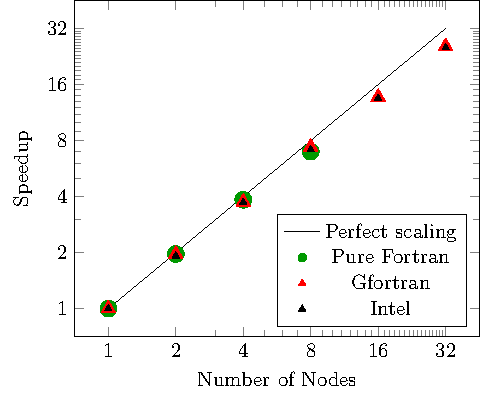
\includegraphics[width=\textwidth]{Figs/PythonScaling/Speedup}
 \caption{\label{fig::Speedup}Speedup when increasing the number of nodes used}
\end{subfigure}
\hspace{.05\textwidth}
\begin{subfigure}[t]{0.45\textwidth}
 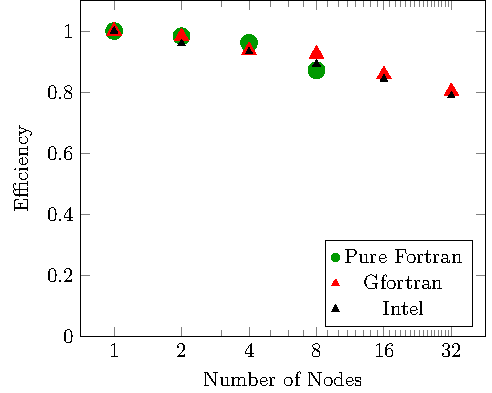
\includegraphics[width=\textwidth]{Figs/PythonScaling/Efficiency}
 \caption{\label{fig::Efficiency}Efficiency with different numbers of nodes}
\end{subfigure}
\caption{\label{fig::Scaling results} Scaling results for the pyccelised version of the code using different compilers}
\end{figure}


\todo{Find more comparisons}

A similar approach to the one described here was used by Latu et al. (1998) \cite{ParallelisationSemi-LagrangianVlasovCodes} with some success although parallel overhead led to limitations on the number of processes which could be used.

\todo{Compare efficiency / moment where overhead dominates}

% 1d: $n^2$ messages
% 
% My 2d: $n_1\cdot n_2$ processes. $n_1n_2^2$ messages. or $n_1^2n_2$ messages.